\documentclass[corpo=12pt,oneside,tipotesi=magistrale,stile=classica]{toptesi}
\usepackage[english,italian]{babel}
\usepackage[utf8]{inputenc}
\usepackage[autostyle,italian=guillemets]{csquotes}
\usepackage[backend=biber,style=ieee]{biblatex}
\usepackage[]{hyperref}
\usepackage{lipsum}
\usepackage{comment}
\usepackage[disable]{todonotes}
\usepackage{listings}
\usepackage{color}
\usepackage{caption}
\usepackage{subcaption}
\usepackage{amsmath}
\usepackage{amsfonts}
\usepackage{multirow}

\definecolor{dkgreen}{rgb}{0,0.6,0}
\definecolor{gray}{rgb}{0.5,0.5,0.5}
\definecolor{mauve}{rgb}{0.58,0,0.82}

\lstset{
	frame=tb,
	aboveskip=3mm,
	belowskip=3mm,
	showstringspaces=false,
	columns=flexible,
	basicstyle={\small\ttfamily},
	numbers=none,
	numberstyle=\tiny\color{gray},
	keywordstyle=\color{blue},
	commentstyle=\color{dkgreen},
	stringstyle=\color{mauve},
	breaklines=true,
	breakatwhitespace=true,
	tabsize=3
}

\addbibresource{Bibliografia/bibliografia.bib}

\hypersetup{
	colorlinks=true,
	linkcolor=black,
	filecolor=magenta,      
	urlcolor=cyan,
}

\excludecomment{commento}
\excludecomment{idee}
\excludecomment{scaletta}


%\includeonly{sommario,Introduzione/intro,DescrizioneAutopilota/px4,Simulazioni/sitl, Appendice/appendice,Bibliografia/bibliografia,SistemaQuadrirotore/modello,SistemaQuadrirotore/leggidicontrollo}

\begin{document}

	\begin{frontespizio*}
		\ateneo{Politecnico di Torino}
		\logosede{polito}
		\CorsoDiLaureaIn{Laurea Magistrale in}
		\corsodilaurea{Ingegneria Aerospaziale}	
		\TesiDiLaurea{Tesi Magistrale}
		\titolo{Software in the loop simulations and Code generation for Unmanned Aerial systems}
		\AdvisorName{Relatore:}
		\relatore{Dr. Elisa Capello}
		\CoAdvisorName{Co-Relatore}
		\secondorelatore{Ing. Davide Carminati}
		\sedutadilaurea{Dicembre 2020}
		\TitoloListaCandidati{Candidato:}
		\candidato{Luigi Sante}
	\end{frontespizio*}

	\sommario
La tesi prevede lo sviluppo del software necessario per il governo di un velivolo a pilotaggio remoto, implementando diversi modelli di controllo e validando il controllore con simulazioni, in cui è stato considerato il software di bordo.

Data la complessità della generazione del software necessario alla guida e controllo dei velivoli di questo tipo, l'approccio più intuitivo, che permette la collaborazione tra diverse figure professionali quali programmatori, ingegneri aerospaziali e meccatronici, risulta essere sicuramente basata sull'utilizzo di una logica progettuale a modelli. Questo tipo di approccio permette di semplificare lo sviluppo del software, concentrando gli sforzi di chi si occupa della creazione dei modelli di controllo sugli aspetti effettivamente importanti della funzionalità di questi, lasciando la complessità della generazione di algoritmi e le relative basi di dati a chi ha maggiore competenza informatica, attraverso lo sviluppo degli strumenti che automatizzano la generazione del codice e la sua compilazione. 
Lo sviluppo del software effettuato in questo modo è accompagnato per ogni passaggio dalla corrispettiva fase di verifica: Model in the loop (MIL), Software in the loop (SIL), Prosessor in the loop (PIL), Hardware in the loop (HIL); aspetto derivato proprio dal classica metodologia di sviluppo del software utilizzante il modello denominato a V, e pienamente solidificato in molti settori industriali.

\'E stato scelto di utilizzare per l'implementazione dell'autopilota il dispositivo PixHawk con il relativo firmware PX4. Lo sviluppo del software avviene quindi specificatamente per questo sistema di prodotti e relativi firmware. Il codice è open-source, permettendo la possibilità di essere studiato e modificato. Il codice si trova ad uno stato abbastanza evoluto nello sviluppo, possedendo tutta una serie di funzionalità già sufficiente per gestire un velivolo a pilotaggio remoto. Nel caso però si voglia inserire un personale modello di guida e controllo o un nuovo stimatore, non sono previsti nativamente strumenti di modellazione, limitando lo sviluppo del software solo alle persone con una competenza informatica elevata, incrementando la complessità di progettazione stessa. In definitiva si ha difficoltà di creazione del codice sorgente partendo da un modello ,esistono comunque gli strumenti per verificare il codice tramite SIL e PIL.

In modo complementare all'utilizzo di PX4, si affianca l'utilizzo di un tool specifico per Simulink, chiamato "Embedded Coder Support Package
for PX4 Autopilots". Grazie a questo tool si permette la generazione del codice in modo automatico partendo dai modelli creati su Simulink e l'inserimento conforme del modulo prodotto all'interno del firmware e delle restanti funzionalità. Integrando quindi gli strumenti di compilazione presenti in PX4 si possono effettuare le simulazioni SIL e PIL, avvicinando lo sviluppo ad una approccio più industriale.

Per testare correttamente il funzionamento di un velivolo a pilotaggio remoto, occorre ricreare in un ambiente simulato il velivolo stesso e le interazioni principali con l'ambiente in cui opera. La scelta dell'ambiente simulato ricade nell'utilizzo di Gazebo. Come anticipato precedentemente la procedura di SIL è nativamente presente nel progetto di PX4. I simulatori selezionabili per questa fase di test sono svariati, il tool di Simulink però limita la scelta ad un simulatore esterno solamente, ovvero JMavSim. Attraverso una procedura particolare però si è reso possibile l'utilizzo di Gazebo, ambiente più versatile e completamente personalizzabile.

Sono stati creati due modelli di controllo delle diverse dinamiche del velivolo e successivamente alla corretta configurazione dei parametri dei controllori, sono stati messi a confronto attraverso simulazioni SIL. Per quando riguarda il controllo di posizione è stato utilizzato un semplice controllore Proportional Iintegral Derivative (PID), mentre per il controllo di quota e di assetto, sono stati utilizzati rispettivamente un controllore PID e un controllore Sliding Mode Control (SMC). L'algoritmo di guida invece prevede la generazione della traiettoria con profili di velocità trapezoidali.

Non è invece stato possibile effettuare correttamente la simulazione PIL a causa di alcuni problemi di comunicazione tra simulatore PixHawk. La trasmissione tra simulatore e autopilota avviene correttamente per quanto riguarda la gestione dei dati dei sensori, ciò non viene altrettanto per quanto riguarda i messaggi da fornire agli attuatori. Questo problema é probabilmente causato dalla differenza sostanziale che c'è tra l'applicazione generata dal tool di Simulink e la logica di base di PX4 nella gestione dei messaggi agli attuatori. Questo aspetto richiede ulteriori indagini in lavori futuri.

\begin{commento}
Inglese

The main purpose of this work is the development of the software necessary for the steering of a UAV (Unmanned Aerial Vehicle) with implementation of different control models and  the validation of the controller with software in the loop.

Given the complexity of the generation of the software necessary to guide and control UAVs (Unmanned Aerial Vehicle), the more intuitive approach, which allows collaboration between different professionals such as programmers, aerospace and mechatronics engineers, is certainly model based design. This type of approach makes it possible to simplify software development, concentrating the efforts the development of control models with focus on important aspects of their functionality, leaving the complexity of generating algorithms and related datastructure to those who have greater IT competence through the development of tools that automate the generation of the code and its compilation.
The software development carried out in this way is validated for each step by the corresponding verification phase: MIL (Model in the loop), SIL (Software in the loop), PIL (Prosessor in the loop), HIL (Hardware in the loop); derived from the classic software development V- model methodology, that is standard in many industrial sectors.

The implementation of the autopilot was made it on the PixHawk 4 device with the relative PX4 firmware. Therefore,the software development takes place specifically for these product systems and related firmware. The code is open-source, allowing the possibility to be studied and modified. The code is fully functional, possessing a whole series of features already sufficient to manage a remotely piloted aircraft. However, if you want to insert a personal GNC (Guidance , navigation and control) model or a new estimator, modeling tools not exist natively, limiting software development only to people with high IT (Information technology) skills, increasing the  overall design complexity itself. Ultimately, it is difficult to create the source code starting from a model, however there are tools included in che sources directory to verify the code through SIL (Software in the loop) and PIL (Prosessor in the loop).

MathWorks has made available a tool called "Embedded Coder Support Package
for PX4 Autopilots " that allows to compensate the aforementioned limitations. Thanks to this tool it is possible to generate the code automatically starting from the models created on Simulink and the insertion of the produced module into the firmware structure with the remaining useful functions. Therefore, integrating the compilation tools included in PX4, SIL (Software in the loop) and PIL (Prosessor in the loop) simulations can be performed, as a more industrial approach.

In order to properly test the operation of the UAV (Unmanned Aerial Vehicle), it is necessary to recreate in a simulated environment the aircraft itself and the main interactions with that. The choice of the simulated environment falls back on Gazebo. As previously mentioned, the SIL (Software in the loop) procedure is natively present in the PX4 project. The simulators that can be selected for this test phase are varied, the Simulink tool however limits the choice to an external simulator only that is JMavSim. However, through a particular procedure, it was possible to use Gazebo, a more versatile and customizable environment.

Two control models of the different dynamics of the aircraft were created and after the correct configuration of the controllers parameters, they were compared through SIL (Software in the loop) simulations. A simple PID (Proportional Iintegral Derivative) controller was used as position controller and a PID (Proportional Integral Derivative) controller and a SMC (Sliding Mode Control) controller respectively were used in order to attitude control. The GNC (Guidance, navigation and control) algorithm foresees a planning trajectory using trapezoidal velocity profile.

The PIL (Prosessor in the loop) simulation could not be performed correctly due to some communication problems between the PixHawk an the simulator. The transmission between the simulator and the autopilot takes place correctly as regards the management of sensor data, this was not the same as regards the messages to be provided to the actuators. This problem was probably caused by the substantial difference between the application generated by the Simulink tool and the basic logic of PX4 in managing messages to the actuators. This aspect requires further investigation in future work.

Abstract

The main purpose of this work is the development of the software necessary for the steering of a Unmanned Aerial Vehicle (UAV) with implementation of different control models and  the validation of the controller with software in the loop.
Given the complexity of the generation of the software necessary to guide and control Unmanned Aerial Vehicles (UAVs), the more intuitive approach, which allows collaboration between different professionals such as programmers, aerospace and mechatronics engineers, is certainly model based design.
The software development carried out in this way is validated for each step by the corresponding verification phase: Model in the loop (MIL), Software in the loop (SIL), Prosessor in the loop (SIL), Hardware in the loop (HIL); derived from the classic software development V-model methodology, that is standard in many industrial sectors.
The implementation of the autopilot was made it on the PixHawk 4 device with the relative PX4 open-source firmware. The code is fully functional, possessing a whole series of features already sufficient to manage a remotely piloted aircraft. However, if you want to insert a personal Guidance , navigation and control (GNC) model or a new estimator, modeling tools not exist natively, limiting software development only to people with high Information technology (IT) skills, increasing the  overall design complexity itself.
MathWorks has made available a tool called "Embedded Coder Support Package
for PX4 Autopilots " that allows to compensate the aforementioned limitations. Thanks to this tool it is possible to generate the code automatically starting from the models created on Simulink and the insertion of the produced module into the firmware structure with the remaining useful functions. Therefore, integrating the compilation tools included in PX4, SIL and PIL simulations can be performed, as a more industrial approach.
The choice of the simulated environment falls back on Gazebo.
Two control models of the different dynamics of the aircraft were created and after the correct configuration of the controllers parameters, they were compared through SIL simulations. A simple Proportional Iintegral Derivative (PID) controller was used as position controller and a PID controller and a Sliding Mode Control (SMC) controller respectively were used in order to attitude control. The GNC algorithm foresees a planning trajectory using trapezoidal velocity profile.
The PIL simulation could not be performed correctly due to some communication problems between the PixHawk an the simulator. The transmission between the simulator and the autopilot takes place correctly as regards the management of sensor data, this was not the same as regards the messages to be provided to the actuators. This problem was probably caused by the substantial difference between the application generated by the Simulink tool and the basic logic of PX4 in managing messages to the actuators. This aspect requires further investigation in future work.


ITALIANO


La tesi prevede lo sviluppo del software necessario per il governo di un velivolo a pilotaggio remoto, implementando diversi modelli di controllo e validando il controllore con simulazioni, in cui è stato considerato il software di bordo.
Data la complessità della generazione del software necessario alla guida e controllo dei velivoli di questo tipo, l'approccio più intuitivo, che permette la collaborazione tra diverse figure professionali quali programmatori, ingegneri aerospaziali e meccatronici, risulta essere sicuramente basata sull'utilizzo di una logica progettuale a modelli.
Lo sviluppo del software effettuato in questo modo è accompagnato per ogni passaggio dalla corrispettiva fase di verifica: Model in the loop (MIL), Software in the loop (SIL), Prosessor in the loop (PIL), Hardware in the loop (HIL); aspetto derivato proprio dal classica metodologia di sviluppo del software utilizzante il modello denominato a V, e pienamente solidificato in molti settori industriali.
E' stato scelto di utilizzare per l'implementazione dell'autopilota il dispositivo PixHawk con il relativo firmware open-source PX4. Il codice si trova ad uno stato evoluto nello sviluppo, possedendo tutta una serie di funzionalità già sufficiente per gestire un velivolo a pilotaggio remoto. Nel caso però si voglia inserire un personale modello di guida e controllo o un nuovo stimatore, non sono previsti nativamente strumenti di modellazione, limitando lo sviluppo del software solo alle persone con una competenza informatica elevata, incrementando la complessità di progettazione stessa.
In modo complementare all'utilizzo di PX4, si affianca l'utilizzo di un tool specifico per Simulink, chiamato "Embedded Coder Support Package
for PX4 Autopilots". Grazie a questo tool si permette la generazione del codice in modo automatico partendo dai modelli creati su Simulink e l'inserimento conforme del modulo prodotto all'interno del firmware e delle restanti funzionalità. Integrando quindi gli strumenti di compilazione presenti in PX4 si possono effettuare le simulazioni SIL e PIL, avvicinando lo sviluppo ad una approccio più industriale.
La scelta dell'ambiente simulato ricade nell'utilizzo di Gazebo.
Sono stati creati due modelli di controllo delle diverse dinamiche del velivolo e successivamente alla corretta configurazione dei parametri dei controllori, sono stati messi a confronto attraverso simulazioni SIL. Per quando riguarda il controllo di posizione è stato utilizzato un semplice controllore Proportional Integral Derivative (PID), mentre per il controllo di quota e di assetto, sono stati utilizzati rispettivamente un controllore PID e un controllore Sliding Mode Control (SMC). L'algoritmo di guida invece prevede la generazione della traiettoria con profili di velocità trapezoidali.
Non è invece stato possibile effettuare correttamente la simulazione PIL a causa di alcuni problemi di comunicazione tra simulatore PixHawk. La trasmissione tra simulatore e autopilota avviene correttamente per quanto riguarda la gestione dei dati dei sensori, ciò non viene altrettanto per quanto riguarda i messaggi da fornire agli attuatori. Questo problema é probabilmente causato dalla differenza sostanziale che c'è tra l'applicazione generata dal tool di Simulink e la logica di base di PX4 nella gestione dei messaggi agli attuatori. Questo aspetto richiede ulteriori indagini in lavori futuri.


\end{commento}

	%\include{ringraziamenti}
	
	\tableofcontents
    \listoftables
	\listoffigures
	
	\mainmatter
	
	\chapter{Introduzione}
La necessità di avere dei velivoli a pilotaggio remoto nasce inizialmente per scopi militari. Il primo velivolo radiocomandato fu infatti in De Haviland 82, adattato per l'addestramento della contraerea con un sistema di pilotaggio remoto attraverso radiocomando \cite{histoDrone}. \'E invece alla sperimentazione riguardante il mondo elicotteristico che si deve la comparsa delle prime configurazioni di quadricottero, un esempio il Jerome-de Bothezat Flying Octopus, velivolo costruito da George de Bothezat nel 1922 \cite{Young}. Ai tempi però questi tipi di configurazione avendo caratteristiche di controllabilità molto carenti e non riuscendo a soddisfare le caratteristiche di peso strutturale e potenze dei motori necessarie non permisero un successivo sviluppo a vantaggio delle configurazioni degli elicotteri così come la conosciamo adesso. Con il successivo avvento della modellistica negli anni '60, lo sviluppo di nuove tecnologie elettroniche e dei materiali, con relativo abbattimento dei costi, si sono potute superare le limitazioni del passato aprendo agli scenari applicativi più svariati oltre a quelli bellici, amatoriali e industriali. Nacquero quindi i primi modelli di droni commerciali.

Attualmente si parla in modo generico di multicottero, comprendendo in questa categoria molteplici configurazioni, tra le quali si è affermata maggiormente grazie alla versatilità e semplicità applicativa quella del quadricottero, configurazione utilizzata anche in questa tesi. Il funzionamento è basato sulla presenza di quattro rotori che generano il sostentamento producendo portanza dalla rotazione. Questi sono disposti in modo che sia anche possibile attraverso l'azionamento differenziale il controllo sul velivolo su tutti quanti i gradi di libertà, principalmente l'assetto e secondariamente a questa la posizione. I rotori sono installati su di una base rigida nella quale oltre al payload sono presenti un sistema di controllo necessario a stabilizzare e comandare il velivolo, i sensori necessari per la determinazione dello stato del velivolo e le interfacce in radiofrequenza per la trasmissione del radio comando e di messaggi più complessi per la navigazione e la telemetria. \'E proprio grazie alla presenza di questi avanzati moduli elettronici miniaturizzati ed estremamente integrati che è stato reso possibile l'utilizzo dei multicotteri altrimenti instabili e ingovernabili \cite{multi2015}. Il sistema infatti è caratterizzato dall'essere un sistema estremamente non lineare con dinamiche accoppiate. Inoltre, avendo in questo caso solo quattro attuazioni, esso risulta essere sottoattuato: meno controlli rispetto ai gradi di libertà \cite{nonlinear2008}.

Vengono riportati i principali vantaggi e svantaggi di questi sistemi \cite{DesTestCarm},\cite{irisquad}.
\paragraph{Vantaggi}
\begin{itemize}
	\item Capacità di mantenere una posizione nello spazio fissa e di decollare verticalmente.
	\item Grande manovrabilità. Il velivolo è in grado di cambiare repentinamente il proprio assetto e la propria velocità.
	\item Sistema molto semplice da costruire e mantenere.
\end{itemize}
\paragraph{Svantaggi}
\begin{itemize}
	\item La durata della batteria è limitata. Risulta limitata l'autonomia di volo.
	\item Il sistema è sottoattuato e non lineare. Questo si traduce in una difficoltà nel essere controllato.
	\item Il payload imbarcabile è relativamente basso.
\end{itemize}

Un aspetto importate da considerare è la presenza dei sensori, senza di questi non sarebbe possibile ricavare attraverso filtraggio e stima, lo stato del velivolo e quindi determinare il controllo da attuare per ottenere la risposta, in termini di posizione e velocità o traiettoria desiderata. I tipici sensori installati sono quelli che permettono la determinazione delle accelerazioni sui tre assi e angolari. Teoricamente queste sei misure se integrate sarebbero sufficienti, ma a causa della intrinseca presenza di rumore ed errori non del tutto eliminabili, si adoperano ulteriori sensori. L'antenna di ricezione del Sistema di posizionamento globale (GPS), un altimetro barometrico e magnetometri, possono compensare i difetti di misurazione, attraverso filtraggio e composizione delle misure \cite{KoksalN2018ALQA}. Nell'applicazione specifica trattata in questa tesi il segnale GPS non è da considerarsi affidabile in quanto, viene ripreso in parte il lavoro di ricerca svolto al Politecnico di Torino \cite{DesTestCarm}, \cite{baseTesi}, ovvero l'uso per applicazioni indoor.


\begin{commento}
citare Development of Hardware-in-the-Loop Simulation Based on Gazebo
	and Pixhawk for Unmanned Aerial Vehicles : assenza di simulink
citare il lavoro di Davide
citare la tesi naval con luso di simulink
citare Implementation of Sliding Mode Fault Tolerant Control on the IRIS+
Quadrotor
\end{commento}

\begin{idee}
\cite{KimJinho2020ACSo} : In questo pubblicazione vengono riassunti vari tipi di controllori che sono stati utilizzati in diverse pubblicazioni. trattato in dettaglio nel capitolo

%\cite{KoksalN2018ALQA} : Necessità di fusione dei sensori per avere una stima corretta del posizionamento del drone nello spazio, in più viene usato un controllore LQR . Qui si fa un test di volo direttamente, che cosa hanno capito?
%
%In questa pubblicazione hanno ottenuto la garanzia di stabilità controllabilità applicando un controllo ottimale.
%Hanno tenuto conto del rumore, confrontando due tipi di filtraggio dei dati dei sensori : Kalman filtro complementare. Il loro scopo era ottimizzare il consumo di batteria attraverso il design ottimale del controllore e path planner. Viene suddiviso il controllo in due livello : alto livello,guidance e posizione; secondo livello attitude e altidue , maggiore interesse in questo . Concentrazione. Due voli sperimentali molto semplici. Drone specifico protetto da struttura di posizione. Io Voglio poterlo fare a rpescindere, cambiare drone.

\cite{ZuluAndrew2014ARoC} : Trade-off tra diversi sistemi di controllo usati in varie pubblicazioni.


\cite{CrazyS} :  Qui si motiva iperchè usare SIL. In questo articolo viene proposto CrasyS una estensione di ROS per modellare , sviluppare e integrare il Quadricottero Crazy flight 2.0 nano nella simulazione basata su Gazebo. Il controllore usa due PID e un generatore del segnale di riferimento. Per validare il sistema viene usato Il toolbox  di MAthWorks Robotics System che collega matlab e simulink a gazebo attraverso messaggi asincroni

Il problema nasce dalla difficoltà di fare volare autonomamente il drone in modo autonomo in contesti particolari come quelli indoor, dove possono verificarsi condizioni imprevedibili.Situazioni critiche. Studiare missioni complesse subito nel mondo reale può essere complicato e richiedere moloto tempo invece la simulazione è molto più semplice, e costare nulla in termini di costi e sicurezza. Si può far schiantare il drone quante volte si vuole. In questo modo dalle simulazioni è possibile testare il sistema in varie condizioni. L'ambiente simulativo è molto versatile e si possono espandere le funzionalità in modo da poter avere più test possibili.

\cite{SIL_design} : Progetto di un sistema di controllo di altitudine sviluppato attraverso le simulazioni fatte in software in the loop. Questo approccio ha permesso di descrivere un procedura di test basati su modelli fisici del sistema. Viene usato una procedura detta chiusura del loop successiva. Il collegamento e lo scambio dei dati con i sensori emulati avviene attraverso protocollo MAVLink. Viene utilizzato DRONEkit e attraverso le sue API, per rendere più facili la generazione di codice del computer compagno con firmware Ardupilot.

\cite{implement} : in questa presentazione del tool di matlab viene presentata la procedura di generazione del codice danda risalto alla necessità di effettuare la validazione seguendo l'approccio model-base. Viene Espressa l'implementazione specifica utilizzando il controllore ixHawk con sistema PX4 . Specificando quale parte del codice viene generato e come questo viene implementato all'interno del firmware dell'hardware. Vengono trttate le funzionalitò del Tool. Viene però usato jMavsim.

\cite{HIL_Dev} : in questa pubblicazione si sviluppa un software per testare l'effettiva comunicazione tra le varie parti del sistema per fare HIL in modo sicuro. viene usato Gazebo pixHawk . Viene sviluppato CAS Control application Software. Viene enfatizzata anche qui la necessità di simulare prima di effettuare test di volo. Riduce il rishio di rompere il sistema, a causa si cadute , fallimenti del sistema malfunzionamento del cotnrollore. Si fa riferimento alla poca versatilità di implementazione di modelli matematici di jmavsim. Gli altri simulatori son molto difficili da modificare in termini di aggiunta di diversi tipi di sensori, per questo si sceglia Gazebo. Gazebo è molto usato in robotica.Prensenta anche la capacità di risolvere la dinamica con il suo motore fisico open Dynamic Engine (ODE), conm grande accuratezza.

\cite{SIL_perform} : In questo lavoro di evidenzia come sia necessario fare SITL. Viene utilizzato il SITL per valutare le performance del sistema di guida e controllo di un UAV, utilizzando un filtro di calman per stimare lo stato del velivolo e un controllo formato da PID

\cite{SIL_Improv} : Questa pubblicazione parla eslicitamente perchè è importate fare SITL. Viene mostrato come alcune criticità della SITL non siano mostrate il MIL. Nele simulazioni vengono considerate missioni complesse. Si fa riferimento esplicito al V-model. Il controllo usato è di tipo PD. In questo lavoro si utilizza ROS con pacchetto RotorS, implementato in Gazebo. Mentre la soluzione è accettabile in MIL, non lo è in SIL, instabilità del controllo.

\cite{Vision_base} : In questo lavoro viene usato PX4 e si fa SITL, utilizzando Gazebo. In Gazebo viene aggiunto un sensore visivo per fare delle simulazioni avanzate sfruttando questa funzionalità.

\cite{SIL_obstacle} : viene validato il sensore LIDAR e la capacità di separazione dagli ostacoli utilizzando un computer di bordo PixHawk , usando un modello simulativo su gazebo in condizioni realistiche. 


%\cite{iso26262} : nella Normativa si fa riferimento alla funcrional Safety. Deriva dalla IEC 61508 standard nel settore specifico elettronico.
%Si utilizza il modello a V : Software integration and verification Software unit verification. 
%
%Facendo software in the loop si possono simulare condizioni pericolose che in un test sperimentale non è possibile fare.
%Si possono verificare i comportamenti in caso di guasti ed errori voluti in fase di simulazione.


\end{idee}




%\begin{idee}
%	Durante la SIT è possibili introdurre fault arbitrari ai fini di testare i meccanismi di sicurezza , simulando la rottura di componenti software e hardware. Il più è possibile valutare sulle macchine target alcuni aspetti di utilizzo delle risorse, questo consente di aumentare la funtional safety del prodotto. In più si può fare back to back comparazione tra modello e codice, garantendo la robustezza del risultato.
%\end{idee}

Nel settore industriare risulta ormai affermata la pratica di progettazione model-based, più precisamente in questo lavoro di tesi si fa riferimento alla fase di generazione del codice, di test e validazione dei componenti software. Prendendo ad esempio il settore automotive viene preso come riferimento da standard di qualità, nella quale si parla di "Software Integration and Unit Verification", come tassello chiave dello sviluppo di software da implementare in dispositivi hardware, seguiti da tutti i documenti redatti per una corretta tranciabilità necessaria ad uno sviluppo coerente e professionale \cite{iso26262}. \'E evidente la necessità di prendere spunto nello sviluppo di questi tipi di prodotto alle pratiche industriali, in modo da soddisfare diversi criteri come la sicurezza. Nella fase di test preliminare del software si possono introdurre situazioni complesse che richiederebbero uno sforzo in termini di tempo e denaro non facilmente affrontabili se non addirittura irrealizzabili, oltre che alla validazione della compatibilità tra il software e l'hardware utilizzato. 


\todo[inline]{motivazione del lavoro}
\todo[inline]{obbiettivo del lavoro}
\todo[inline]{Perchè è importate fare SITL e PITL invece che flight test}
Come riportato nella stessa guida di PX4 \cite{px4Firmware}, le simulazioni sono il modo più sicuro e rapido per testare il codice, prima di avere il vero e proprio quadricottero. Dal settore automotive si può capire l'importanza di un approccio model based con corrispettive fasi di validazione, \cite, vantaggi nella progettazione semplificando la descrizione del problema e nell'automazione della fase di testing del prodotto. 



\section{Organigramma della tesi}
La tesi è suddivisa, oltre a questo capitolo introduttivo, in tre capitoli:
\begin{itemize}
	\item \textbf{Sistema Quadrirotore:} In questo capitolo verrà trattato nel dettaglio il sistema quadrirotore. Nello specifico verranno considerati il modello matematico, le leggi di controllo adottate e gli algoritmi di guida.
	\item \textbf{Descrizione Autopilota :} Verranno trattati i dettagli del sistema scelto per l'implementazione. Varranno descritti in questo capitolo i dettagli del drone, l'autopilota scelto con il corrispettivo firmware e gli strumenti messi a disposizione per i test, con le modifiche effettuate.
	\item \textbf{Simulazioni : } In questo ultimo capitolo verranno messi a confronto attraverso le simulazioni due differenti sistemi di controllo e le conclusioni. L'ultima parte del capitolo riguarderà il lavoro svolto sulle simulazioni PIL e i problemi riscontrati e possibili studi futuri.
\end{itemize}	
	
	%\chapter{Sistema Quadrirotore}
	\chapter{Sistema Quadrirotore}

\section{Modello matematico}


	\section{Leggi di controllo}
\subsection{Controllore PID}

\begin{figure}
	\centering
	\includegraphics[width=1\textwidth]{DescrizioneAutopilota/Figure/completopid}
	\caption{Modello di controllo completo PID}
\end{figure}

\begin{figure}
	\centering
	\includegraphics[width=1\textwidth]{DescrizioneAutopilota/Figure/attitudecontrollerpid}
	\caption{Modello di controllo d' assetto PID}
\end{figure}

\begin{figure}
	\centering
	\includegraphics[width=1\textwidth]{DescrizioneAutopilota/Figure/altitudecontrollerpid}
	\caption{Modello di controllo di altitudine PID}
\end{figure}

\begin{figure}
	\centering
	\includegraphics[width=1\textwidth]{DescrizioneAutopilota/Figure/positioncontrollerpid}
	\caption{Modello di controllo di posizione PID}
\end{figure}

\begin{figure}
	\centering
	\includegraphics[width=0.5\textwidth]{DescrizioneAutopilota/Figure/armpid}
	\caption{Modello di gestione dei segnali di armamento}
\end{figure}

\todo[inline]{Inserire le tabelle con i parametri}
	\section{Algoritmi di guida}

\begin{idee}
	\cite{ElikerKaram2018AOPf}
	\cite{baseTesi}
	\cite{Mendoza-SotoJoséLuis2018Cgpc}
	\cite{PathPlannigOverview}
	
	
	\cite{YangLiang2016SoR3} : 
	
	\cite {Literature3dPath} : 
	
	La necessità è quella di avere autonomia nello spostamento senza l'intervento dell'uomo, determinando autonomamente il percorso da seguire.
	Tra gli obbiettivi di pianificazione del percorso c'è anche quello di evitare gli ostacoli possibili per questioni di sicurezza.
	Nel contesto degli UAV il problema è un problema tridimensionale.
	
	La soluzione a questo tipo di problema è estremamente complessa.
	
	Si può suddividere il problema in 2 parti fondamentali:
	
	1. Percezione e modellazione dell'ambiente
	2. Applicazione dell'algoritmo di pianificazione
	
	Non è necessario però che la pianificazione si sempre accompagnata da una ottimizazione, alcune volte basta che questa colleghi i due punti nello spazio.
	Si distingue in pianificazione del persorso e pianificazione del percorso ottimo se si vuole ottimizzare una certa funzione di costo oppure no.
	
	Sussiste una differenza tra pianificazione del percorso e della traiettoria. La pianificazione del percorso cerca solo un a curva o una sequenza di curve che colleghino due punti nello spazio, mentre la pianificazione della traiettoria prevede di determinare anche come questa debba essere percorsa, descrivendo in modo cinematico e dinamico, attraverso la valutazione di questi nella ricerca della soluzione.
	
	Si possono classificare gli algoritmi di pianificazione dei percorsi in 5 categorie.
	
	1. Algoritmi basati sul campionamento:
		Questi algoritmi richiedono la conoscenza a priori di informazioni sull'ambiente e una rappresenzazione matematica di questo. Si prevede di dividere l'ambiente in nodi o celle o altre forme. Avviene poi una ricerca attraverso una ricerca casuale. Questa categoria si può suddividere a sua volta in altre 2 categorie : attive e passive. Attive  si intende algoritmi che esploraro rapidamente in modo casuale per trovare il percorso migliore. Passivi algoritmi che si occupano di cercare la soluzione da percorsi già presenti come su di una mappa.
		
	2. Algoritmi basati sui nodi
		Questi algoritmi sono basati sull'utilizzo di nodi appartenenti ad un grafo scomposto, ricercando le soluzioni gia eseguite.
		
	3. Algoritmi basati su modelli matematici
		Questi metodi modellano l'ambiente  e il sistema e il sistema e modellano la funzione di costo con i limiti e vincoli per ottenere la soluzione ottimale. Equazioni e disequazioni
		
	
	
\end{idee}
	\section{Implementazioni del controllo utilizzate}
	
	%\chapter{Descrizione Autopilota}
	\chapter{Descrizione Autopilota}


\section{Descrizione del drone}


\todo[inline]{Descrizione del drone e dell'hardware dell'autopilota}
	\section{Descrizione del firmware PX4 Autopilot}
Il firmware utilizzato nelle simulazioni di software in the loop e processor in the loop è il PX4 Autopilot \cite{px4Firmware}, \cite{px4Guide}.
	
Questo software mette a disposizione diverse funzionalità per avere un sistema di gestione e controllo robusto e affidabile, implementato in diversi tipi di sistemi. L'implementazione non è quindi specifica solo a mezzi aerei di qualsiasi configurazione, ma anche a velicoli di terra, marini e razzi. Il software è open-source e vanta del contributo di parecchi sviluppatori, dagli esperti del settore a contributi di livello accademico. Lo sviluppo open-source permette quindi di aggiungere o modificare le funzionalità messe a disposizione in modo da soddisfare le proprie esigenze e arricchire il progetto generico di nuove funzionalità utili ad altri. Il sistema operativo sulla quale viene eseguito materialmente il codice può essere Nuttx o Linux/MacOS la cui distinzione principale in questa applicazione è solo nella gestione di task e thread.

Il sistema operativo Nuttx è un sistema RTOS (Real-Time Operating System) è svilupato appositamente per implementazioni embedeed. Essendo sviluppato per un contesto specifico ha tutte le caratteristiche necessarie per essere eseguito in sistemi che devono avere prestazioni migliori con poche risorse disponibili. Vengono utilizzati gli standard POSIX e ANSI \cite{Nuttx}. Inoltre, sono implementate funzionalità di programmazione concorrenziale per l'esecuzione di processi in parallelo. Le funzionalità del firmware vengono eseguite in questo sistema come task separati e ogni task può eseguire diversi thread.
Nell'implementazione su sistemi Linux/MacOS invece i moduli sono eseguiti come thread del processo principale, non c'è quindi una distinzione tra threads e tasks, oltre a non essere ottimizzato per sistemi embedeed.


\subsection{Architettura del software}
Il firmware è principalmente suddiviso in due categorie di moduli:
\begin{itemize}
	\item \textbf{Flight stack} : composta dalla parte che stima lo stato del sistema e il relativo controllo
	\item \textbf{Middleware} : composta dalle interfacce che collegano i vari moduli interni di PX4 tra di loro e verso l'esterno, con la possibilità di integrare gli hardware utilizzati.
\end{itemize}

Il sistema quindi separa le varie funzionalità in moduli separati, eseguiti in modo indipendente che scambiano i dati e comandi tra di loro e con l'esterno attraverso messaggi asincroni.
Nella figura \ref{fig:px4.architettura} è riportato lo schema di alto livello del software di PX4 e la sua modularità.

\begin{figure}
	\centering
	\includegraphics[width=0.8\textwidth]{DescrizioneAutopilota/Figure/PX4_Architecture}
	\caption{Architettura del codice di PX4 Autopilot, \cite{px4Guide}}
	\label{fig:px4.architettura}
\end{figure}
\subsubsection{Flight stack}
Il flight stack, mostrato in figura \ref{fig:px4.flightstack} è l'insieme di moduli che si occupano della stima dello stato del sistema e di tutti le funzionalità per il controllo,la guida e la navigazione. Esiste anche un modulo per interfacciarsi con il volo manuale attraverso radiocomando.
	\begin{figure}[ht]
	\centering
	\includegraphics[width=1\textwidth]{DescrizioneAutopilota/Figure/PX4_High-Level_Flight-Stack}
	\caption{Architettura del flight stack di PX4, \cite{px4Guide}}
	\label{fig:px4.flightstack}
\end{figure}
\paragraph{Estimator}
L'estimator è il modulo che prendendo i dati da uno o più sensori determina lo stato attuale del velivolo. E' possibile selezionare diversi tipi di estimato, quello selezionato in questo caso è uno stimatore con filtro di Kalman.
\paragraph{Controller}
Si occupa di prendere in input i vari punti della pianificazione e confrontarli con lo stato attuale determinato dell'estimator. In questo modo vengono determinati i segnali di comando di output che saranno poi elaborati dal mixer. Questa funzionalità è implementata da più moduli, suddividendo la dinamica lenta e la dinamica veloce del drone. Verrà disabilitata la sua funzionalità per sostituirla con l'applicazione sviluppata su Simulink.
\paragraph{Mixer}
Il mixer si occupa di tradurre i segnali del comandi normalizzati di rollio, imbardata, beccheggio e manetta, da consegnare all'hardware che genera gli impulsi pwm utilizzati per il controllo del motore.
\subsubsection{Middleware}
Questo insieme di moduli si occupa invece di tutte le comunicazioni interne tra processi e tra PX4 e il mondo esterno. \'E composta principalmente dai driver per i sensori, i canali di comunicazione verso l'esterno e il bus di trasmissione di messaggi attraverso $\micro$ORB e MAVLink. In questo contesto ricade anche  la connessione con un simulatore per testare il codice generato nelle varie fasi di validazione.
\subsection{Strumenti per lo sviluppo del codice}
Il sistema operativo utilizzato per lo sviluppo è Ubuntu 18.04.5 LTS, nella quale è stato installato MATLAB 2020a. Viene inoltre installato il tool "Embeded Coder Support Package for PX4 Autopilots", seguendo la guida, \cite{PX4MATLAB}. La versione di Ubuntu  installata però non è pienamente compatibile in quanto no presenta di default il software necessario al lancio delle simulazioni da parte di Simulink, ovvero "xterm", che va installato manualmente. La versione di PX4 utilizzata è quella prevista dalla guida \cite{PX4MATLAB}, ovvero la versione "1.8.0". Risulta inoltre necessario installare anche la versione di Java 8 e ROS-Melodic con il modulo di Gazebo.

L'intero codice del firmware PX4 viene messo a disposizione attraverso la piattaforma github, \cite{PX4FIRMWARE}. Il progetto contiene all'interno le toolchain necessarie per compilare il sistema nei vari sistemi operativi. Agendo sulle varie possibili configurazioni di compilazione è possibile modificare e aggiunge delle funzionalità. Modificando le impostazioni di compilazione si può generare il programma finale da caricare ed eseguire sull'autopilota.
Sono presenti anche delle configurazioni per effettuare l'analisi e la verifica del codice generato attraverso l'utilizzo di un ambiente simulato. I simulatori che presentano una configurazione di base sono : Gazebo, jMAVSim , AirSim, Xplane. Per quanto riguarda questa tesi, verrà utilizzato il software Gazebo sfruttando parzialmente il codice già presente e adottando alcune modifiche. Nulla vieta comunque di poter collegare un simulatore diverso attraverso la creazione di un interfaccia dati con il firmware. Infatti, la connessione viene effettuata attraverso UDP o seriale, utilizzando su essa il protocollo MAVLink.

Per la generazione del codice sorgente da implementare nel firmware PX4, si fa utilizzo delle funzionalità aggiunte a MATLAB/Simulink dal tool "Embeded Coder Support Package for PX4 Autopilots", \cite{PX4MATLAB}. Dopo l'installazione di questo pacchetto vengono aggiunti alla libreria standard di Simulink, alcuni blocchetti utili all'interfacciamento con le restanti parti del firmware di PX4. Attraverso l'utilizzo di messaggi $\micro$ORB avvengono infatti le comunicazioni con i moduli eseguiti parallelamente alla configurazione del firmware: stimatore, sensori, attuatori ecc.

Nella creazione del modello in Simulink, si è tenuto conto del fatto che i dati necessari al controllo, venissero prelevati dallo stimatore di default di PX4, a differenza del lavoro svolto precedentemente in \cite{DesTestCarm}, nella quale si sono implementati le funzioni dei sensori e uno stimatore specifico.

Attraverso l'uso dei messaggi passati dal Firmware a Simulink quindi si sono implementati i controllori come spiegato in dettaglio nel capilo precedente. Nella Figura (\ref{fig:in}), viene mostrato l'implementazione su simulink necessaria a leggere lo stato del drone.

\begin{figure}
	\centering
	\includegraphics[width=0.8\textwidth]{DescrizioneAutopilota/Figure/IN}
	\caption{Interfaccia di input del modulo di controllo implementato su Simulink}
	\label{fig:in}
\end{figure}

Analogamente avviene il collegamento in output del sistema di controllo con l'apposito modulo della libreria, Figura (\ref{fig:out}).

\begin{figure}
	\centering
	\includegraphics[width=0.6\textwidth]{DescrizioneAutopilota/Figure/OUT}
	\caption{Interfaccia di output del modulo di controllo implementato su Simulink}
	\label{fig:out}
\end{figure}

Utilizzando quindi questi moduli in input e output, il Coder è in grado generare il codice sorgente, incapsularlo in un modulo di PX4 e compilarlo. Da questo si ottiene quindi un file eseguibile con il sistema PX4 compilato e integrato in esso il controllo implementato. 

Nativamente il tool di Simulink sopracitato non permette l'utilizzo dell'ambiente Gazebo, ma solamente il simulatore jMavSim. Per questo è stato studiato il processo di lancio della simulazione integrato nel tool e la documentazione sui collegamenti tra il firmware PX4 e Gazebo nelle simulazioni SIL effettuate senza utilizzare Simulink. Attraverso la scrittura di uno script, presente in appendice, si è superata questa limitazione, rendendo possibile l'utilizzo di Gazebo per effettuare le simulazioni SIL. In Figura (\ref{fig:ig:INTERSIL}), viene mostrata la configurazione utilizzata per effettuare le simulazioni SIL. Come è possibile osservare nel caso si compili il codice per effettuare SIL, viene compilato all'interno del firmware un modulo che ha lo scopo specifico di interfacciare il simulatore con il Firmware. Il controllore utilizzato è integrato come modulo all'interno del firmware stesso.

\begin{figure}
	\centering
	\includegraphics[width=0.8\textwidth]{DescrizioneAutopilota/Figure/INTERSIL}
	\caption{Configurazione per effettuare le simulazioni SIL}
	\label{fig:ig:INTERSIL}
\end{figure}



	\section{Gazebo}
\label{section:gazebo}

\todo[inline]{Descrizione della simulazione in gazebo e dell'adattamento al problema della tesi}

	%\chapter{Simulazioni}
	\section{Simulazione SITL}
\subsection{PID}
\subsubsection{STEP}
\todo[inline]{Tabella dei waypoints}
\begin{figure}
	\centering
	\includegraphics[width=0.5\textwidth]{Simulazioni/Figure/STEPaltitudecontrolposPID}
	\caption{Risposta con PID al segnale STEP : quota}
\end{figure}

\begin{figure}
	\centering
	\includegraphics[width=0.5\textwidth]{Simulazioni/Figure/STEPaltitudecontrolvelPID}
	\caption{Risposta con PID al segnale STEP : rateo di salita}
\end{figure}

\begin{figure}
	\centering
	\includegraphics[width=0.5\textwidth]{Simulazioni/Figure/STEPpwmPID}
	\caption{Risposta con PID al segnale STEP : PWM}
\end{figure}

\clearpage
\subsection{SMC}
\subsubsectio{STEP}
\begin{figure}
	\centering
	\includegraphics[width=0.5\textwidth]{Simulazioni/Figure/STEPaltitudecontrolposSMC}
	\caption{Risposta con PID al segnale STEP : quota}
\end{figure}

\begin{figure}
	\centering
	\includegraphics[width=0.5\textwidth]{Simulazioni/Figure/STEPaltitudecontrolvelSMC}
	\caption{Risposta con PID al segnale STEP : rateo di salita}
\end{figure}

\begin{figure}
	\centering
	\includegraphics[width=0.5\textwidth]{Simulazioni/Figure/STEPpwmSMC}
	\caption{Risposta con PID al segnale STEP : PWM}
\end{figure}

\clearpage
\subsection{Confronto}
	\section{Simulazioni MIL}
\todo[inline]{Citare il lavoro fatto da davide per i sensori e lo stimatore usato in quel caso}
\todo[inline]{I parametri usati in MIL e SIL per i controllori sono gli stessi}
\todo[inline]{Il controllori risultano iperattivi in MIL rispetto al SIL}

\subsection{PID}
\subsubsection{SNAKE}
\begin{figure}
	\centering
	\begin{subfigure}{0.45\textwidth}
		\centering
		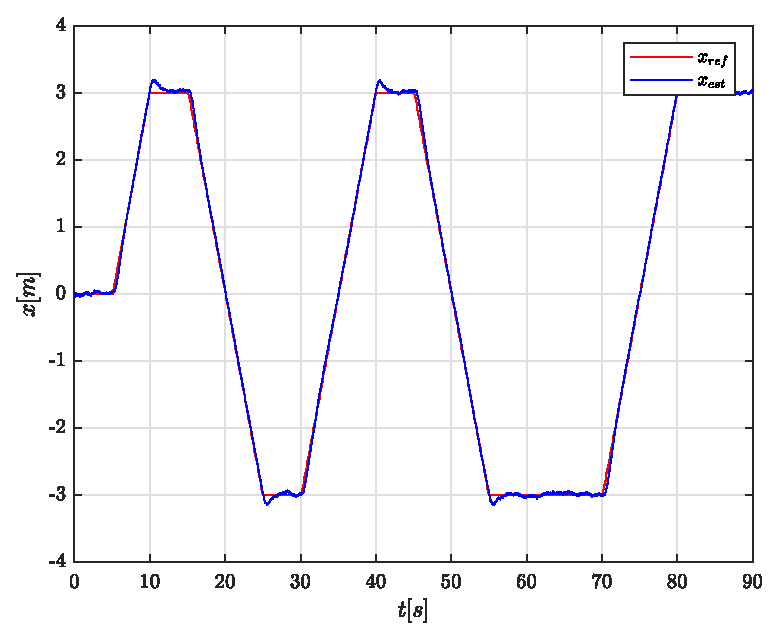
\includegraphics[width=1\textwidth]{Simulazioni/Figure/PID/SNAKE_MIL/PositionControlXPos}
		\caption{Controllo posizione lungo x}
	\end{subfigure}
	\hfill
	\begin{subfigure}{0.45\textwidth}
		\centering
		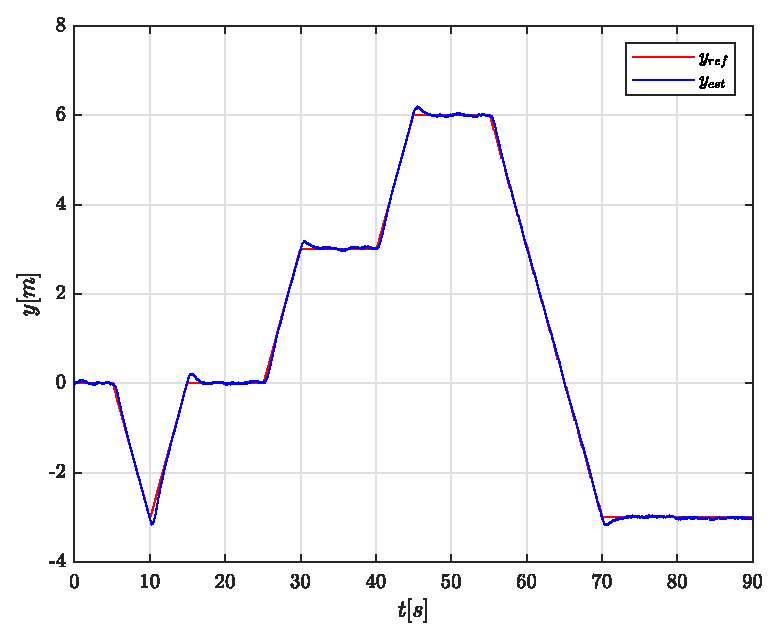
\includegraphics[width=1\textwidth]{Simulazioni/Figure/PID/SNAKE_MIL/PositionControlYPos}
		\caption{Controllo posizione lungo y}
	\end{subfigure}
	\\
	\begin{subfigure}{0.45\textwidth}
		\centering
		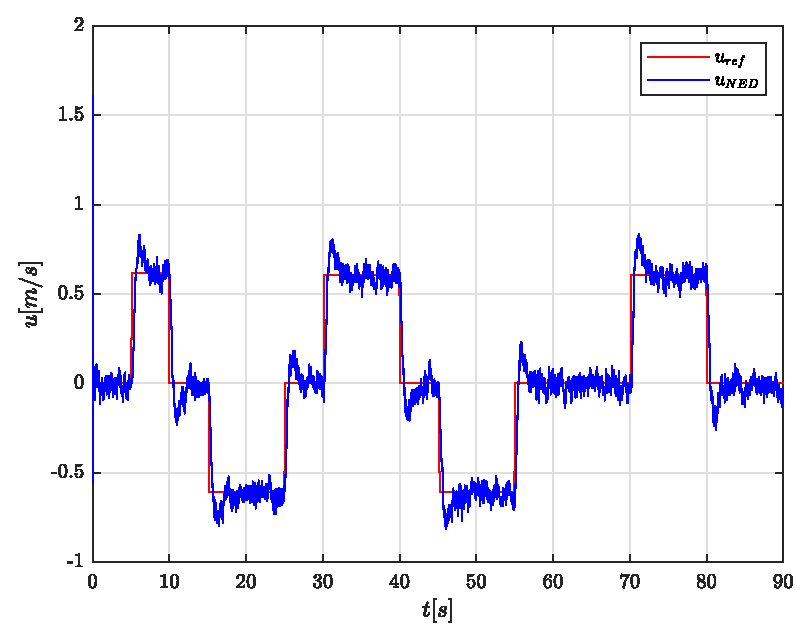
\includegraphics[width=1\textwidth]{Simulazioni/Figure/PID/SNAKE_MIL/PositionControlXVel}
		\caption{Controllo velocità lungo x}
	\end{subfigure}
	\hfill
	\begin{subfigure}{0.45\textwidth}
		\centering
		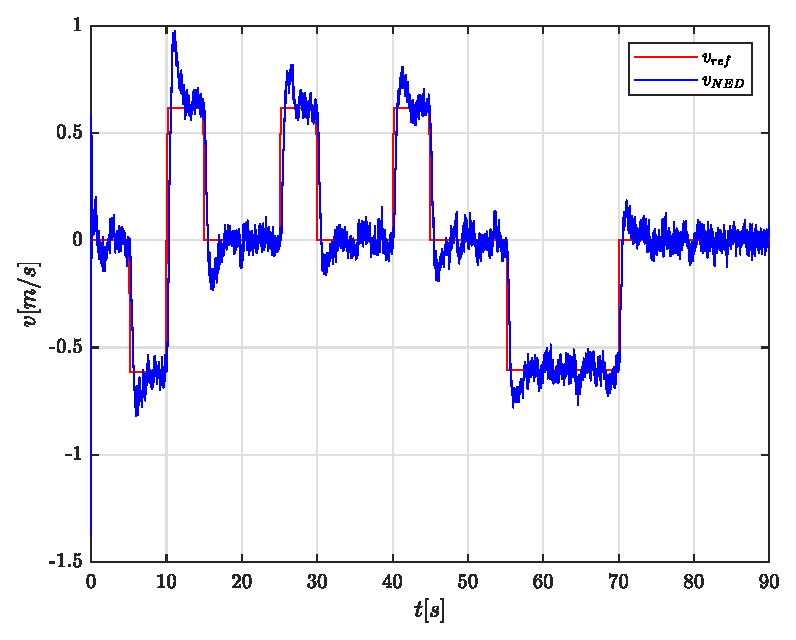
\includegraphics[width=1\textwidth]{Simulazioni/Figure/PID/SNAKE_MIL/PositionControlYVel}
		\caption{Controllo velocità lungo y}
	\end{subfigure}
	\caption{Risposta nella simulazione MIL in posizione con controllore interno PID al comando SNAKE}
\end{figure}

\begin{figure}
	\centering
	\begin{subfigure}{0.45\textwidth}
		\centering
		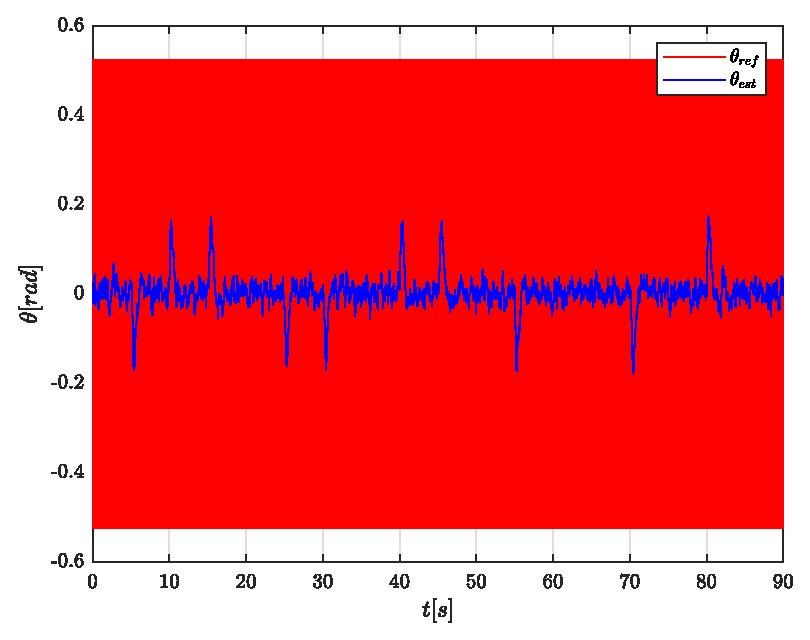
\includegraphics[width=1\textwidth]{Simulazioni/Figure/PID/SNAKE_MIL/AttitudeControlPitch}
		\caption{Controllo beccheggio}
	\end{subfigure}
	\hfill
	\begin{subfigure}{0.45\textwidth}
		\centering
		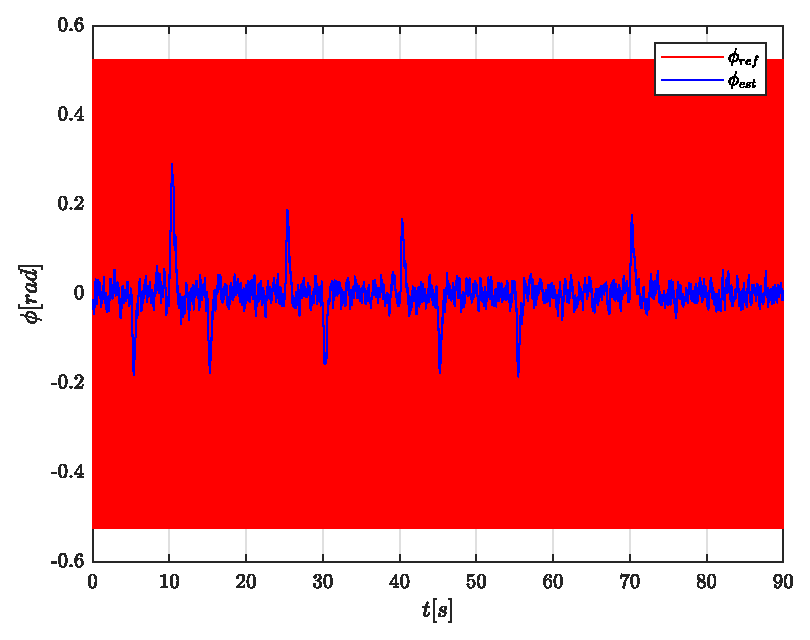
\includegraphics[width=1\textwidth]{Simulazioni/Figure/PID/SNAKE_MIL/AttitudeControlRoll}
		\caption{Controllo rollio}
	\end{subfigure}
	\hfill
	\begin{subfigure}{0.45\textwidth}
		\centering
		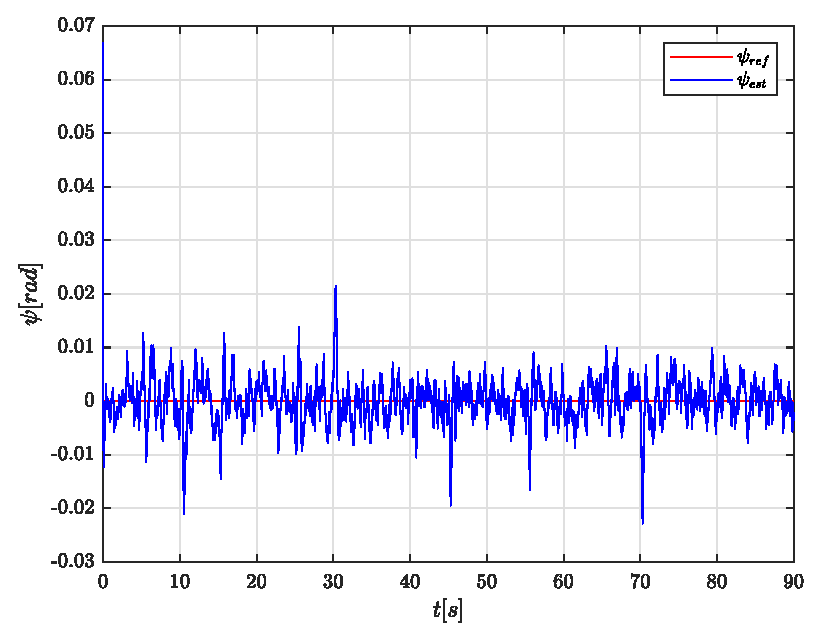
\includegraphics[width=1\textwidth]{Simulazioni/Figure/PID/SNAKE_MIL/AttitudeControlYaw}
		\caption{Controllo imbardata}
	\end{subfigure}
	\caption{Risposta dell' assetto nella simulazione MIL con controllore interno PID al comando SNAKE}
\end{figure}


\begin{figure}
	\centering
	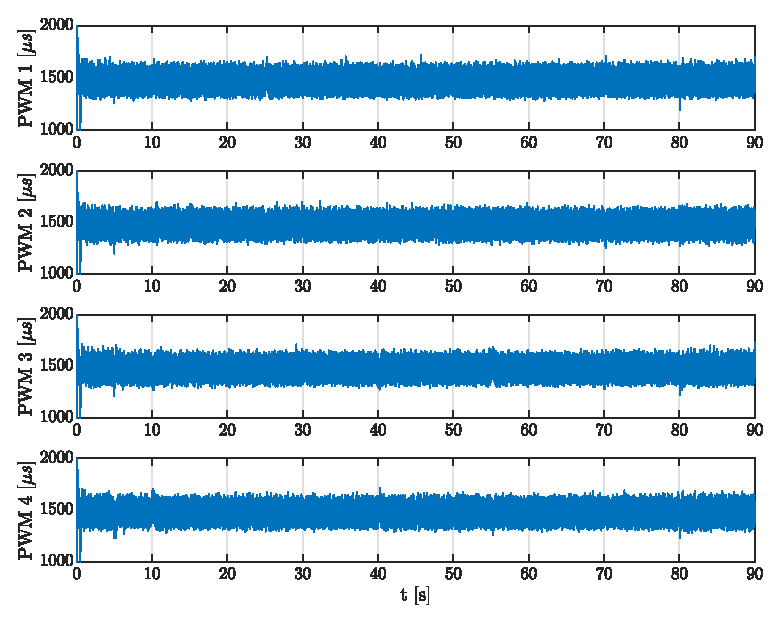
\includegraphics[width=0.5\textwidth]{Simulazioni/Figure/PID/SNAKE_MIL/PWM}
	\caption{Segnali PWM nella simulazione MIL del controllore PID al segnale SNAKE}
\end{figure}
\begin{figure}
	\centering
	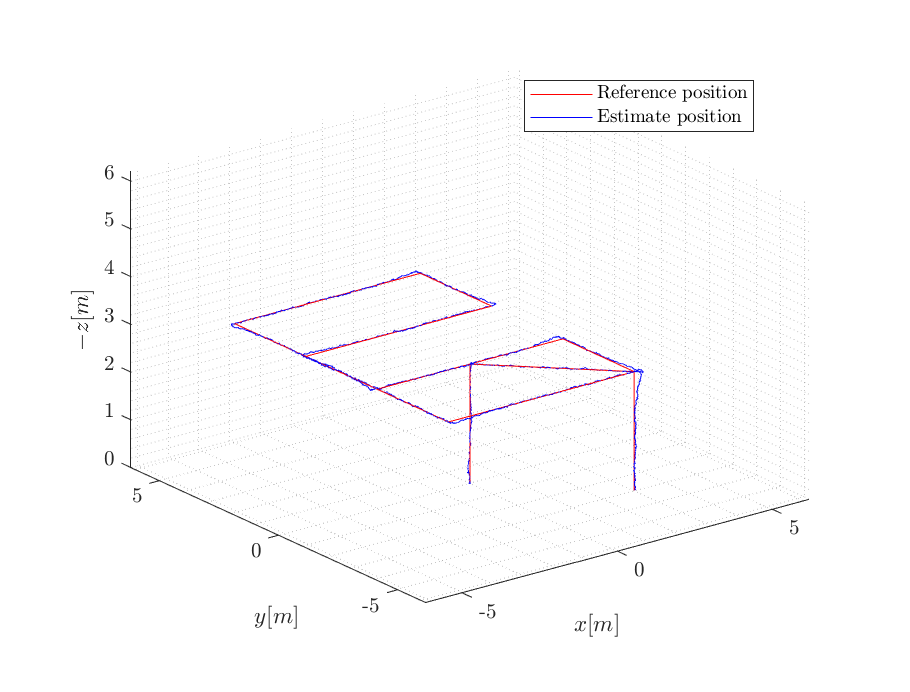
\includegraphics[width=1\textwidth]{Simulazioni/Figure/PID/SNAKE_MIL/Trajectory}
	\caption{Traiettoria percorsa nella simulazione MIL con controllore PID al segnale SNAKE}
\end{figure}

\clearpage
\subsection{SMC}
\subsubsection{SNAKE}
\begin{figure}
	\centering
	\begin{subfigure}{0.45\textwidth}
		\centering
		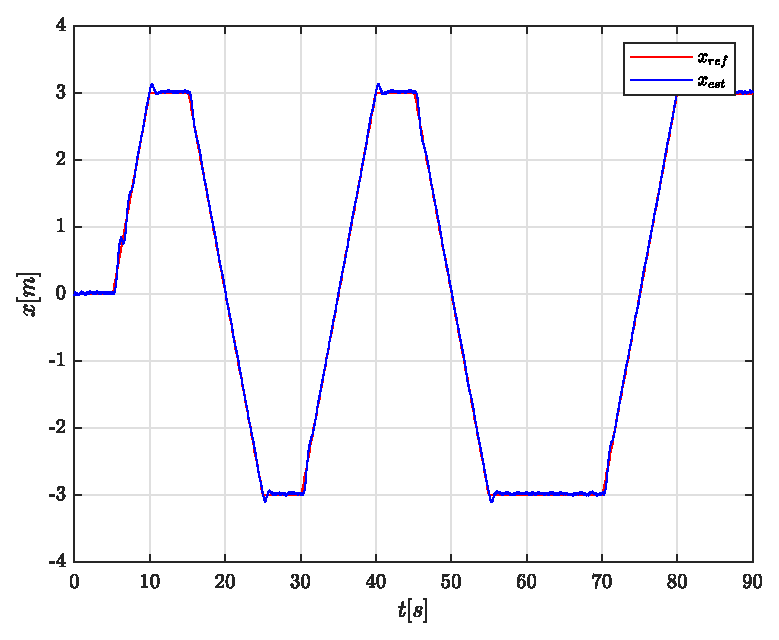
\includegraphics[width=1\textwidth]{Simulazioni/Figure/SMC/SNAKE_MIL/PositionControlXPos}
		\caption{Controllo posizione lungo x}
	\end{subfigure}
	\hfill
	\begin{subfigure}{0.45\textwidth}
		\centering
		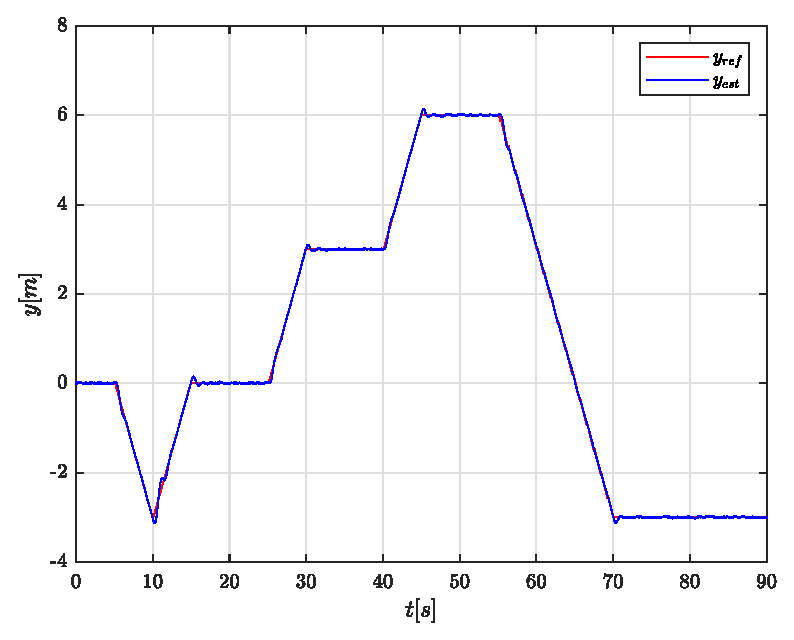
\includegraphics[width=1\textwidth]{Simulazioni/Figure/SMC/SNAKE_MIL/PositionControlYPos}
		\caption{Controllo posizione lungo y}
	\end{subfigure}
	\\
	\begin{subfigure}{0.45\textwidth}
		\centering
		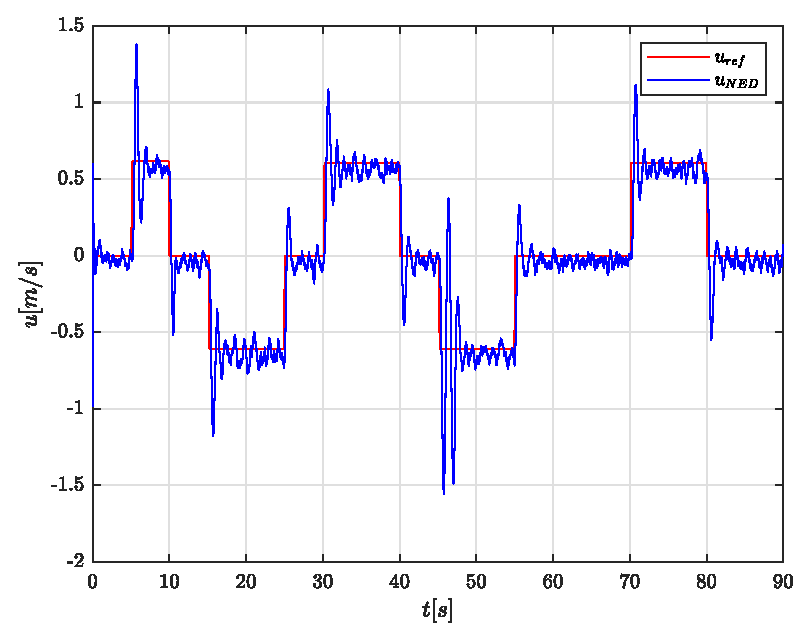
\includegraphics[width=1\textwidth]{Simulazioni/Figure/SMC/SNAKE_MIL/PositionControlXVel}
		\caption{Controllo velocità lungo x}
	\end{subfigure}
	\hfill
	\begin{subfigure}{0.45\textwidth}
		\centering
		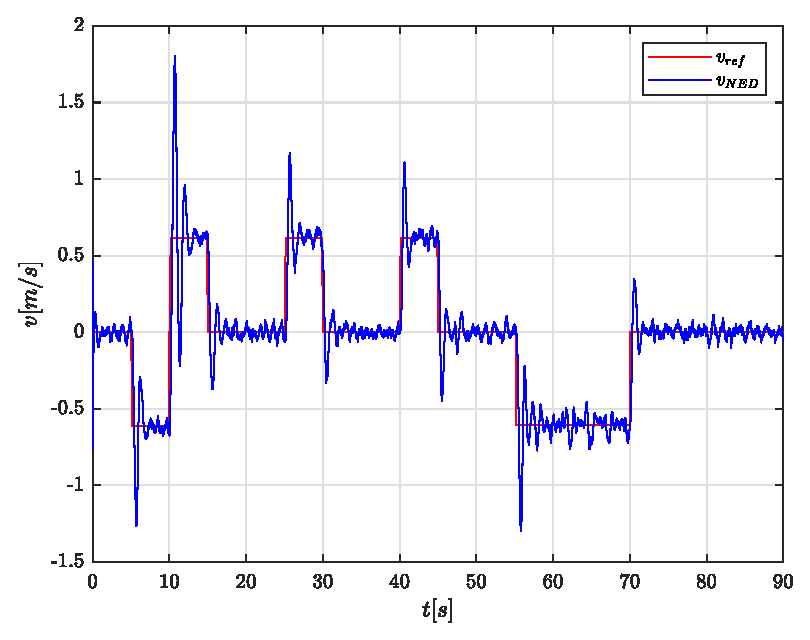
\includegraphics[width=1\textwidth]{Simulazioni/Figure/SMC/SNAKE_MIL/PositionControlYVel}
		\caption{Controllo velocità lungo y}
	\end{subfigure}
	\caption{Risposta in posizione nella simulazione MIL con controllore interno SMC al comando SNAKE}
\end{figure}

\begin{figure}
	\centering
	\begin{subfigure}{0.45\textwidth}
		\centering
		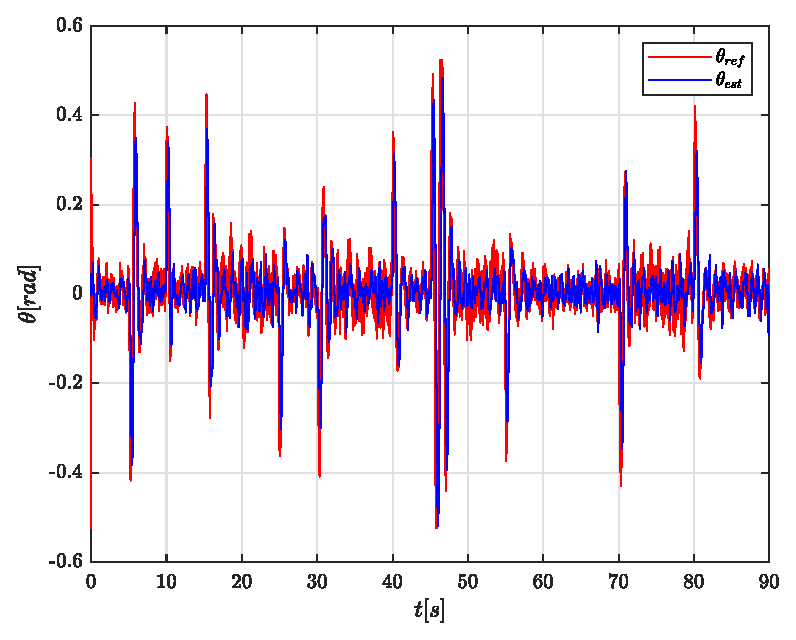
\includegraphics[width=1\textwidth]{Simulazioni/Figure/SMC/SNAKE_MIL/AttitudeControlPitch}
		\caption{Controllo beccheggio}
	\end{subfigure}
	\hfill
	\begin{subfigure}{0.45\textwidth}
		\centering
		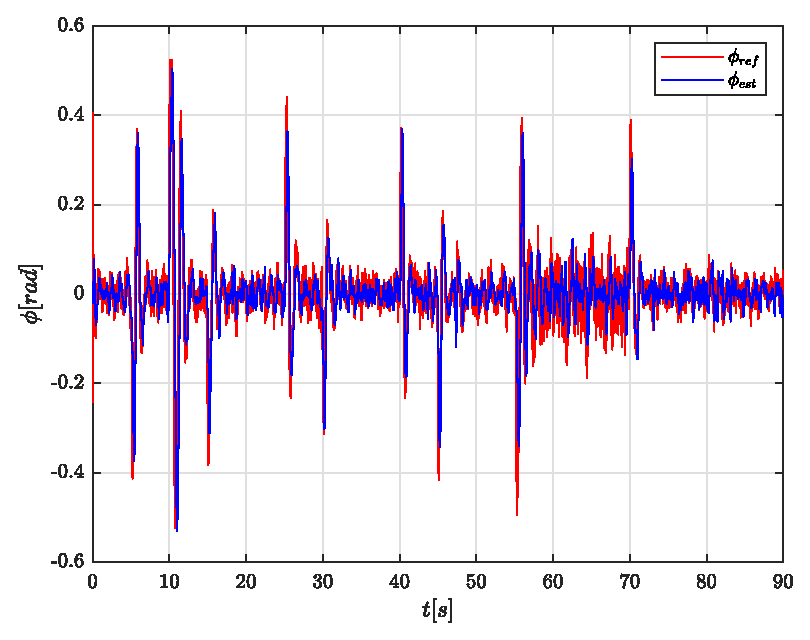
\includegraphics[width=1\textwidth]{Simulazioni/Figure/SMC/SNAKE_MIL/AttitudeControlRoll}
		\caption{Controllo rollio}
	\end{subfigure}
	\hfill
	\begin{subfigure}{0.45\textwidth}
		\centering
		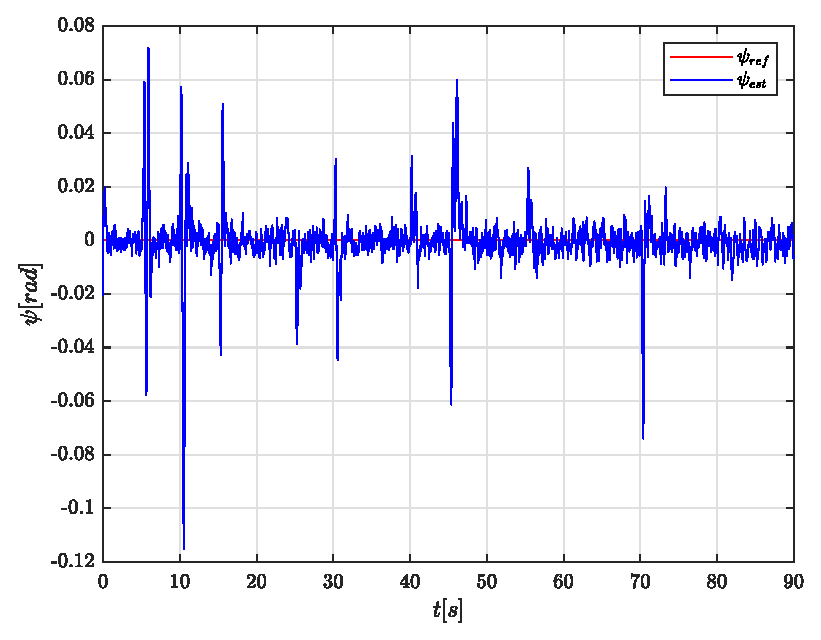
\includegraphics[width=1\textwidth]{Simulazioni/Figure/SMC/SNAKE_MIL/AttitudeControlYaw}
		\caption{Controllo imbardata}
	\end{subfigure}
	\caption{Risposta dell' assetto nella simulazione MIL con controllore interno SMC al comando SNAKE}
\end{figure}


\begin{figure}
	\centering
	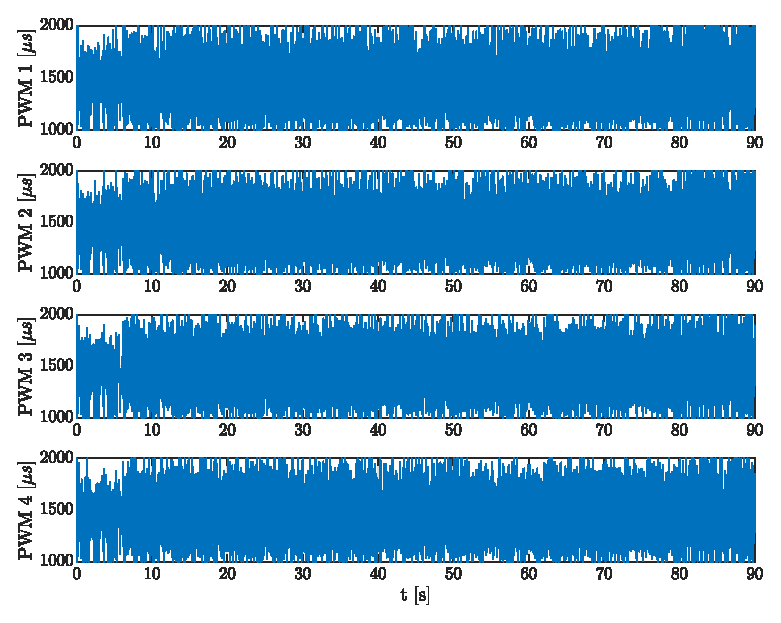
\includegraphics[width=0.5\textwidth]{Simulazioni/Figure/SMC/SNAKE_MIL/PWM}
	\caption{Segnali PWM del controllore SMC al segnale SNAKE}
\end{figure}
\begin{figure}
	\centering
	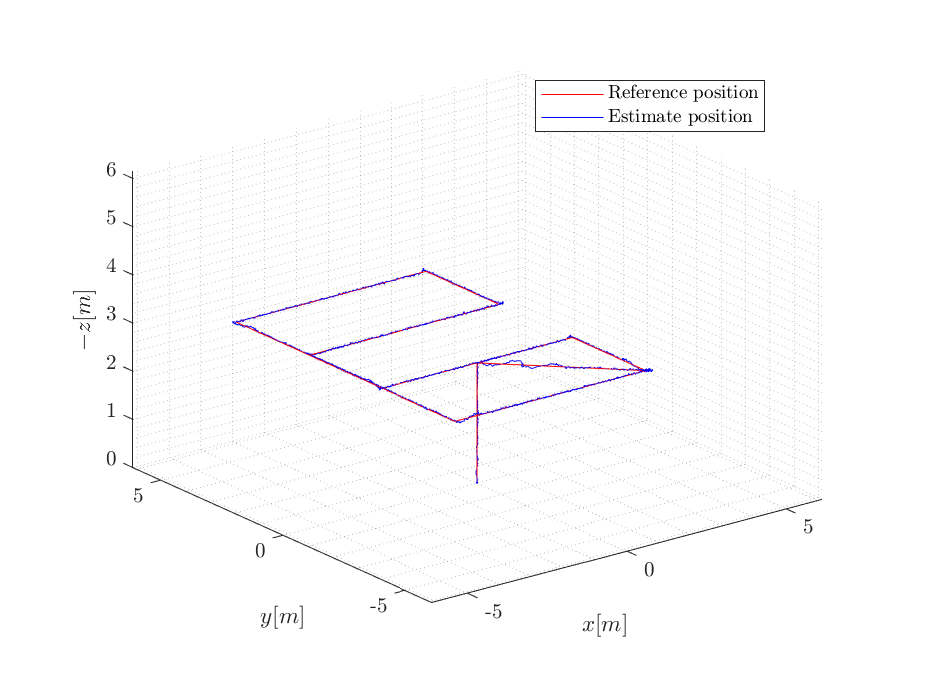
\includegraphics[width=1\textwidth]{Simulazioni/Figure/SMC/SNAKE_MIL/Trajectory}
	\caption{Traiettoria percorsa con controllore SMC nella simulazione MIL al segnale SNAKE}
\end{figure}
\subsection{Confronto}
\todo[inline]{Confronto tra MIL e SIL per il segnale SNAKE}
\todo[inline]{Il controllore SMC risulta più robusto. Il Controllore PID non si sarebbe mai ottenuto partendo dal MIL perchè in quel tipo di simulazione ha una risposta pessima. Importanza della SIL per valutare l'effetto introdotto dall'implementazione software per correggere i parametri di reogalzione trovati in MIL}

	\section{Simulazioni PIL}
\todo[inline]{Descrizione del metodo di collegamento}
\todo[inline]{Parlare dell'importanza dello script di boot e fare riferimento all'appendice}
\todo[inline]{Descrizione dei successi e fallimenti nella simulazione}
\todo[inline]{Input correttamente comunicati dal simulatore}
\todo[inline]{Problema con gli output non comunicati al simulatore}

	\section{Conclusione}
\todo[inline]{Descrizione complessiva del lavoro, risultati finali complessivi}
\todo[inline]{Sviluppi futuri}
\todo[inline]{Sviluppo di un software per collegare correttamente in simulazione PIL}
\todo[inline]{Migliorare il simulatore Gazebo aggiungendo dettagli e modelli di sensori per applicazioni indoor}


 %lavori futuri
	
	\backmatter
	\chapter{Appendice}
\subsection{Modifiche nel codice dei plugin di Gazebo}

\lstset{language=c++}
\begin{lstlisting}
//gazebo_motor_model.cpp

...

//Leggo i parametri dal file di impostazione

getSdfParam<double>(_sdf, "ForceQuadraticCoefficent", force_quadratic_coefficent_, force_quadratic_coefficent_);
getSdfParam<double>(_sdf, "ForceLinearCoefficent", force_linear_coefficent_, force_linear_coefficent_);
getSdfParam<double>(_sdf, "ForceCostant", force_costant_, force_costant_);
getSdfParam<double>(_sdf, "ForceMinRpmFitting", force_min_rpm_fitting_, force_min_rpm_fitting_);

getSdfParam<double>(_sdf, "MomentQuadraticCoefficent", moment_quadratic_coefficent_, moment_quadratic_coefficent_);
getSdfParam<double>(_sdf, "MomentLinearCoefficent", moment_linear_coefficent_, moment_linear_coefficent_);
getSdfParam<double>(_sdf, "MomentCostant", moment_costant_, moment_costant_);
getSdfParam<double>(_sdf, "MomentMinRpmFitting", moment_min_rpm_fitting_, moment_min_rpm_fitting_);

...

//Aggiungo modifica forma quadratica
double force = std::isgreater(std::abs(real_motor_velocity),force_min_rpm_fitting_)*
(real_motor_velocity * real_motor_velocity * force_quadratic_coefficent_ 
+ std::abs(real_motor_velocity)* force_linear_coefficent_ + force_costant_);
if (force<0) force=0;

link_->AddRelativeForce(ignition::math::Vector3d(0, 0, force));

ignition::math::Vector3d drag_torque(0, 0, -turning_direction_ *
std::isgreater(std::abs(real_motor_velocity),
moment_min_rpm_fitting_)*(real_motor_velocity * 
real_motor_velocity * moment_quadratic_coefficent_ + 
std::abs(real_motor_velocity) * moment_linear_coefficent_+ moment_costant_));

...

ignition::math::Vector3d drag_torque_parent_frame = pose_difference.Rot().RotateVector(drag_torque);
parent_links.at(0)->AddRelativeTorque(drag_torque_parent_frame);

...

\end{lstlisting}

\lstset{language=XML}
\begin{lstlisting}
<!-- drone.sdf-->

...

<plugin name='front_left_motor_model' filename='libgazebo_motor_model.so'>
<robotNamespace/>
<jointName>rotor_3_joint</jointName>
<linkName>rotor_3</linkName>
<turningDirection>cw</turningDirection>
<maxRotVelocity>2000</maxRotVelocity>
<commandSubTopic>/gazebo/command/motor_speed</commandSubTopic>
<motorNumber>3</motorNumber>
<motorSpeedPubTopic>/motor_speed/3</motorSpeedPubTopic>
<rotorVelocitySlowdownSim>10</rotorVelocitySlowdownSim>
<ForceQuadraticCoefficent>1.1632e-5</ForceQuadraticCoefficent>
<ForceLinearCoefficent>-0.0202</ForceLinearCoefficent>
<ForceCostant>8.1513</ForceCostant>
<ForceMinRpmFitting>1000</ForceMinRpmFitting>
<MomentQuadraticCoefficent>2.6604e-7</MomentQuadraticCoefficent>
<MomentLinearCoefficent>-4.6797e-4</MomentLinearCoefficent>
<MomentCostant>0.2046</MomentCostant>
<MomentMinRpmFitting>1000</MomentMinRpmFitting>

...

\end{lstlisting}

\subsection{Script per il lancio delle simulazioni SIL}

\lstset{language=bash}
\begin{lstlisting}
#File : sil.h
#!/bin/bash

export GAZEBO_MODEL_DATABASE_URI=""

sim=$1

Firmware=$(realpath .)

cp posix-configs/SITL/init/ekf2/iris posix-configs/SITL/init/ekf2/sim

if [ "$#" -lt 1 ]
then
echo Specificare il simulatore : jmavsim , gazebo
exit 1
fi

if [ "$sim" == "gazebo" ] 
then
cd build/posix_sitl_default/build_gazebo
if [ "$(ls -A .)" ]
then
echo "Makefile gia' presente"
else
echo "Creazione makefile"
cmake $Firmware/Tools/sitl_gazebo
fi
echo "Esecuzione makefile"
make
cd $Firmware/build/posix_sitl_default
else
cd $Firmware/build/posix_sitl_default
fi

$Firmware/Tools/sitl_run.sh $Firmware/build/posix_sitl_default/px4  posix-configs/SITL/init/ekf2 none $sim sim $Firmware $Firmware/build/posix_sitl_default
\end{lstlisting}

\subsection{Script per il lancio delle simulazioni PIL}
\lstset{language=bash}
\begin{lstlisting}
#File : pil.h
#!/bin/bash

export GAZEBO_MODEL_DATABASE_URI=""

src_path=$(realpath .)
build_path=$src_path/build/nuttx_px4fmu-v5_default

mkdir $build_path/build_gazebo

cd $build_path/build_gazebo
if [ "$(ls -A .)" ]
then
echo "Makefile gia' presente"
else
echo "Creazione makefile"
cmake $src_path/Tools/sitl_gazebo
fi
echo "Esecuzione makefile"
make
cd $build_path

source $src_path/Tools/setup_gazebo.bash ${src_path} ${build_path}

gazebo --verbose ${src_path}/Tools/sitl_gazebo/worlds/sim_pil.world
\end{lstlisting}

\subsection{Script personalizzato di avvio del PixHawk}
\lstset{language=bash}
\begin{lstlisting}
#File : rc.txt
#
# Start the ORB (first app to start)
#
uorb start

#
# Load parameters
#
set PARAM_FILE /fs/microsd/params

param select $PARAM_FILE
param load

param reset_nostart RC* COM_FLTMODE* LND_FLIGHT_T_*

#
# Start system state indicator
#
rgbled start

# FMUv5 may have both PWM I2C RGB LED support
rgbled_pwm start

if param compare BAT_N_CELLS 0
then
param set BAT_N_CELLS 3
fi

param set COM_RC_IN_MODE 1
param set SYS_AUTOSTART 1001
param set SYS_HITL 1
param set NAV_RCL_ACT 0

#
# Set default values (modificati)
#
set VEHICLE_TYPE mc
set MIXER quad_x
set MIXER_AUX quad_x
set OUTPUT_MODE hil # set hil
set PWM_OUT 1234
set PWM_RATE 50
set PWM_DISARMED 100
set PWM_MIN 1000
set PWM_MAX 2000
set PWM_AUX_OUT yes
set PWM_AUX_RATE 50
set PWM_ACHDIS none
set PWM_AUX_DISARMED 100
set PWM_AUX_MIN 1000
set PWM_AUX_MAX 2000
set FAILSAFE_AUX no
set MK_MODE none
set FMU_MODE pwm
set AUX_MODE pwm
set FMU_ARGS "-t" #USE FMU TASK
set MAVLINK_F xnone
set MAVLINK_COMPANION_DEVICE /dev/ttyS2
set MAV_TYPE 2 #quad x
set FAILSAFE no
set USE_IO no
set LOGGER_BUF 64 #PX4FMUV5

sh /etc/init.d/1001_rc_quad_x.hil #set hil and quad x mixer

dataman start 
sensors start -h
commander start --hil
send_event start
load_mon start

#
# Check if UAVCAN is enabled, default to it for ESCs
#
if param greater UAVCAN_ENABLE 2
then
set OUTPUT_MODE uavcan_esc
fi

if fmu mode_$FMU_MODE $FMU_ARGS
then
else
echo "FMU start failed" >> $LOG_FILE
fi

if pwm_out_sim start
then
else
echo "pwm_out_sim start failed" >> $LOG_FILE
fi

px4flow start &

# Load mixer and configure outputs
sh /etc/init.d/rc.interface

ekf2 start      
px4_simulink_app start

usleep 10000

mavlink start -d /dev/ttyS1 -b 921600 -m config -x

mavlink boot_complete
\end{lstlisting}


\subsection{Modelli Simulink}
\begin{figure}
	\centering
	\includegraphics[width=1\textwidth]{DescrizioneAutopilota/Figure/completopid}
	\caption{Modello di controllo completo PID}
\end{figure}

\begin{figure}
	\centering
	\includegraphics[width=1\textwidth]{DescrizioneAutopilota/Figure/attitudecontrollerpid}
	\caption{Modello di controllo d' assetto PID}
\end{figure}

\begin{figure}
	\centering
	\includegraphics[width=1\textwidth]{DescrizioneAutopilota/Figure/altitudecontrollerpid}
	\caption{Modello di controllo di altitudine PID}
\end{figure}

\begin{figure}
	\centering
	\includegraphics[width=1\textwidth]{DescrizioneAutopilota/Figure/positioncontrollerpid}
	\caption{Modello di controllo di posizione PID}
\end{figure}

\begin{figure}
	\centering
	\includegraphics[width=0.5\textwidth]{DescrizioneAutopilota/Figure/armpid}
	\caption{Modello di gestione dei segnali di armamento}
\end{figure}
	\include{Bibliografia/bibliografia}
	
\end{document}